\chapter{Aksjomaty oddzielania}
\label{ch:topog-oddzielanie}

\noindent\textbf{Cel rozdziału.}
W dotychczasowych konstrukcjach nie wymagaliśmy, aby różne punkty
miały różne otoczenia ani by punkty i zbiory domknięte można było
oddzielić zbiorami otwartymi. Tymczasem własności te wpływają na
jednoznaczność granic, zachowanie funkcji ciągłych i konstrukcje ilorazowe.
Wprowadzimy aksjomaty $T_0$, $T_1$, $T_2$, regularność, całkowitą
regularność i normalność. Wykażemy także lemat Urysohna
i twierdzenie Tietzego o przedłużeniu. Każde założenie podamy jawnie: samych pojęć
regularności i normalności nie utożsamiamy odpowiednio z aksjomatami
$T_3$ i $T_4$.

\section{Rozróżnianie punktów: $T_0$, $T_1$ i Hausdorff}
\label{sec:topog-t0-t1-t2}

\begin{definicja}[Aksjomaty $T_0$, $T_1$, $T_2$]
\label{def:topog-t0-t1-t2}
Niech $(X,\tau)$ będzie przestrzenią topologiczną.
\begin{enumerate}[label=(\roman*)]
\item $X$ spełnia \emph{aksjomat $T_0$} (jest przestrzenią
Kołmogorowa), gdy dla każdych dwóch różnych punktów $x,y\in X$
istnieje zbiór otwarty zawierający dokładnie jeden z nich.
\item $X$ spełnia \emph{aksjomat $T_1$}, gdy dla każdych $x\ne y$
istnieją zbiory otwarte $U,V\subseteq X$ takie, że
$x\in U$, $y\notin U$ oraz $y\in V$, $x\notin V$.
\item $X$ spełnia \emph{aksjomat $T_2$} (jest przestrzenią
Hausdorffa), gdy dla każdych $x\ne y$ istnieją rozłączne
zbiory otwarte $U,V\subseteq X$ takie, że $x\in U$ i $y\in V$.
\end{enumerate}
Dla przestrzeni pustej i jednoelementowej wszystkie trzy warunki
są spełnione: nie istnieje para różnych punktów.
\end{definicja}


\begin{figure}[htbp]
\centering
\begin{minipage}[t]{.48\textwidth}
\centering
\textbf{Warunek $T_1$}\\[2pt]
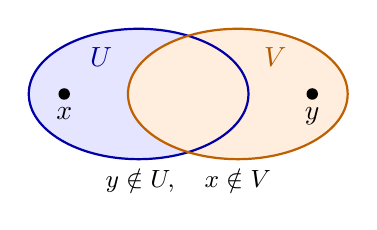
\begin{tikzpicture}[scale=.90]
  \fill[blue!10] (-.7,0) ellipse (1.55 and .92);
  \fill[orange!13] (.7,0) ellipse (1.55 and .92);
  \draw[blue!65!black,thick] (-.7,0) ellipse (1.55 and .92);
  \draw[orange!75!black,thick] (.7,0) ellipse (1.55 and .92);
  \fill (-1.75,0) circle (2.3pt);
  \fill (1.75,0) circle (2.3pt);
  \node[below] at (-1.75,-.06) {$x$};
  \node[below] at (1.75,-.06) {$y$};
  \node[blue!60!black] at (-1.23,.52) {$U$};
  \node[orange!70!black] at (1.23,.52) {$V$};
  \node[font=\small] at (0,-1.22) {$y\notin U,\quad x\notin V$};
\end{tikzpicture}
\end{minipage}\hfill
\begin{minipage}[t]{.48\textwidth}
\centering
\textbf{Warunek $T_2$}\\[2pt]
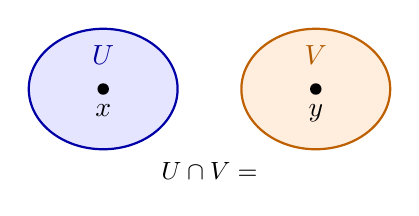
\begin{tikzpicture}[scale=.90]
  \fill[blue!10] (-1.5,0) ellipse (1.05 and .85);
  \fill[orange!13] (1.5,0) ellipse (1.05 and .85);
  \draw[blue!65!black,thick] (-1.5,0) ellipse (1.05 and .85);
  \draw[orange!75!black,thick] (1.5,0) ellipse (1.05 and .85);
  \fill (-1.5,0) circle (2.3pt);
  \fill (1.5,0) circle (2.3pt);
  \node[below] at (-1.5,-.08) {$x$};
  \node[below] at (1.5,-.08) {$y$};
  \node[blue!60!black] at (-1.5,.48) {$U$};
  \node[orange!70!black] at (1.5,.48) {$V$};
  \node[font=\small] at (0,-1.15) {$U\cap V=\varnothing$};
\end{tikzpicture}
\end{minipage}
\caption{Porównanie aksjomatów $T_1$ i $T_2$. Po lewej
\emph{wybrane} otoczenie $U$ punktu $x$ nie zawiera $y$,
a wybrane otoczenie $V$ punktu $y$ nie zawiera $x$;
otoczenia te mogą się przecinać. Po prawej możemy wybrać
otoczenia rozłączne. Rysunki przedstawiają schematy warunków,
a nie konkretne topologie.}
\label{fig:topog-t1-t2-porownanie}
\end{figure}

\begin{stwierdzenie}[Pierwsze implikacje]
\label{prop:topog-t2-t1-t0}
Dla dowolnej przestrzeni topologicznej $X$ zachodzą implikacje
$T_2\Rightarrow T_1\Rightarrow T_0$.
\end{stwierdzenie}
\begin{proof}
Jeśli $x\in U$, $y\in V$ i $U\cap V=\varnothing$, to
$y\notin U$ i $x\notin V$, co daje $T_1$. Z kolei przy założeniu
$T_1$ jeden ze zbiorów otwartych przewidzianych w definicji
rozróżnia punkty w sensie $T_0$.
\end{proof}

\begin{przyklad}[Przestrzeń Sierpińskiego]
\label{ex:topog-sierpinski-oddzielanie}
Niech $X=\{0,1\}$ i $\tau=\{\varnothing,\{1\},X\}$.
Otwarty zbiór $\{1\}$ rozróżnia $0$ i $1$, więc $X$ jest $T_0$.
Nie ma jednak otwartego zbioru zawierającego $0$ i niezawierającego
$1$, ponieważ jedynym otoczeniem otwartym punktu $0$ jest $X$.
Przestrzeń nie spełnia $T_1$, a tym bardziej $T_2$.
\end{przyklad}

\begin{twierdzenie}[Kryterium za pomocą singletonów]
\label{thm:topog-t1-singletony}
Przestrzeń topologiczna $X$ jest $T_1$ wtedy i tylko wtedy,
gdy każdy zbiór jednoelementowy $\{x\}$, $x\in X$, jest domknięty.
\end{twierdzenie}
\begin{proof}
Załóżmy $T_1$ i ustalmy $x\in X$. Dla każdego $y\ne x$
istnieje otwarty zbiór $U_y$ zawierający $y$ i niezawierający
$x$. Stąd
\[
X\setminus\{x\}=\bigcup\{U\in\tau:x\notin U\},
\]
więc dopełnienie singletonu jest otwarte, a singleton domknięty.
Równość jest prawdziwa również, gdy $X=\{x\}$: obie strony są puste.

Odwrotnie, niech wszystkie singletony będą domknięte i $x\ne y$.
Wówczas otwarte zbiory $X\setminus\{y\}$ oraz
$X\setminus\{x\}$ zawierają odpowiednio $x$ i $y$
i nie zawierają drugiego punktu, co daje $T_1$.
\end{proof}

\begin{wniosek}[Skończone przestrzenie $T_1$]
\label{cor:topog-skonczone-t1}
Skończona przestrzeń topologiczna jest $T_1$ wtedy i tylko wtedy,
gdy ma topologię dyskretną.
\end{wniosek}
\begin{proof}
W przestrzeni $T_1$ każdy singleton jest domknięty, a każdy
podzbiór zbioru skończonego jest skończoną sumą singletonów.
Wszystkie podzbiory są więc domknięte, a zatem także otwarte.
Odwrotnie, w topologii dyskretnej singletony są domknięte.
\end{proof}

\begin{przyklad}[Topologia koskończona]
\label{ex:topog-koskonczona-t1-nie-t2}
Niech $X$ będzie nieskończony z topologią koskończoną:
zbiory otwarte to $\varnothing$ i zbiory o skończonym dopełnieniu.
Każdy singleton jest domknięty, zatem $X$ jest $T_1$.
Jeżeli $U,V$ są niepustymi otwartymi, to
$X\setminus(U\cap V)=(X\setminus U)\cup(X\setminus V)$
jest skończony; ponieważ $X$ jest nieskończony,
$U\cap V\ne\varnothing$. Nie można więc rozdzielić
żadnej pary różnych punktów rozłącznymi zbiorami otwartymi:
$X$ nie jest Hausdorffa.
\end{przyklad}

\begin{stwierdzenie}[Przekątna i aksjomat Hausdorffa]
\label{prop:topog-przekatna-hausdorff}
Niech $X$ będzie przestrzenią topologiczną, a $X\times X$
ma topologię iloczynu. Wówczas $X$ jest Hausdorffa wtedy i tylko
wtedy, gdy przekątna $\Delta_X=\{(x,x):x\in X\}$ jest domknięta
w $X\times X$.
\end{stwierdzenie}
\begin{proof}
Jeśli $X$ jest Hausdorffa i $(x,y)\notin\Delta_X$, to $x\ne y$.
Wybierzmy rozłączne otwarte $U\ni x$ i $V\ni y$.
Prostokąt $U\times V$ jest otwarty, zawiera $(x,y)$ i nie przecina
$\Delta_X$. Takie prostokąty pokrywają dopełnienie przekątnej,
które jest więc otwarte.

Odwrotnie, niech $\Delta_X$ będzie domknięta i $x\ne y$.
Dopełnienie przekątnej jest otwarte i zawiera $(x,y)$.
Z kryterium bazy topologii iloczynu, udowodnionego
w rozdziale 04, istnieją otwarte $U\ni x$,
$V\ni y$ takie, że $(x,y)\in U\times V\subseteq
(X\times X)\setminus\Delta_X$. Gdyby $z\in U\cap V$,
to $(z,z)\in U\times V\cap\Delta_X$, sprzeczność.
Zatem $U\cap V=\varnothing$.
\end{proof}

\begin{twierdzenie}[Zgodność odwzorowań na zbiorze gęstym]
\label{thm:topog-rownosc-na-gestym}
Niech $X$ będzie przestrzenią topologiczną, $Y$ przestrzenią
Hausdorffa, a $f,g\colon X\to Y$ odwzorowaniami ciągłymi.
Wówczas zbiór $E=\{x\in X:f(x)=g(x)\}$ jest domknięty.
Jeśli ponadto $D\subseteq X$ jest gęsty w $X$ i $f=g$ na $D$,
to $f=g$ na całym $X$.
\end{twierdzenie}
\begin{proof}
Odwzorowanie $h=(f,g)\colon X\to Y\times Y$ jest ciągłe:
jego współrzędne są ciągłe, a więc stosujemy własność
uniwersalną iloczynu z rozdziału 04.
Z poprzedniego stwierdzenia $\Delta_Y$ jest domknięta,
zatem $E=h^{-1}(\Delta_Y)$ jest domknięty.
Jeśli $D\subseteq E$ i $\overline D=X$, to
$X=\overline D\subseteq E$, a więc $E=X$.
\end{proof}

\begin{uwaga}[Warunek Hausdorffa ma znaczenie]
Niech $Y$ będzie przestrzenią Sierpińskiego i niech
$X=Y$, $D=\{1\}$. Zbiór $D$ jest gęsty, ponieważ jedynym
niepustym otwartym zbiorem zawierającym $0$ jest $Y$.
Odwzorowanie identycznościowe $f\colon X\to Y$ i odwzorowanie
stałe $g(x)=1$ są ciągłe, zgadzają się na $D$, lecz nie
zgadzają się w punkcie $0$. Pokazuje to konieczność
warunku oddzielania w poprzednim twierdzeniu.
\end{uwaga}

\section{Regularność i aksjomat $T_3$}
\label{sec:topog-regularnosc}

\begin{definicja}[Regularność i aksjomat $T_3$]
\label{def:topog-regularnosc-t3}
Przestrzeń topologiczna $X$ jest \emph{regularna}, jeżeli dla
każdego zbioru domkniętego $F\subseteq X$ i każdego $x\in X\setminus F$
istnieją rozłączne zbiory otwarte $U,V\subseteq X$ takie, że
$x\in U$ i $F\subseteq V$.
Przestrzeń spełnia \emph{aksjomat $T_3$}, gdy jest jednocześnie
regularna i $T_1$.
\end{definicja}

\begin{stwierdzenie}[Kryterium zwężania otoczeń]
\label{prop:topog-regularnosc-zwezanie}
Przestrzeń topologiczna $X$ jest regularna wtedy i tylko wtedy,
gdy dla każdego $x\in X$ i każdego otwartego $W\subseteq X$
zawierającego $x$ istnieje otwarty $U\subseteq X$ taki, że
$x\in U\subseteq\overline U\subseteq W$.
\end{stwierdzenie}
\begin{proof}
Załóżmy regularność i przyjmijmy $F=X\setminus W$.
Ponieważ $F$ jest domknięty i $x\notin F$, istnieją rozłączne
otwarte $U\ni x$ i $V\supseteq F$. Domknięty zbiór
$X\setminus V$ zawiera $U$, stąd
$\overline U\subseteq X\setminus V\subseteq W$.

Odwrotnie, dla domkniętego $F$ i $x\notin F$ zastosujmy warunek
do otwartego $W=X\setminus F$. Otrzymamy
$x\in U\subseteq\overline U\subseteq X\setminus F$.
Zbiory $U$ i $V=X\setminus\overline U$ są otwarte i rozłączne,
przy czym $F\subseteq V$.
\end{proof}

\begin{wniosek}[$T_3$ pociąga za sobą $T_2$]
\label{cor:topog-t3-t2}
Każda przestrzeń $T_3$ jest Hausdorffa.
\end{wniosek}
\begin{proof}
Dla $x\ne y$ singleton $\{y\}$ jest domknięty na mocy
aksjomatu $T_1$ i twierdzenia \ref{thm:topog-t1-singletony}.
Regularność rozdziela punkt $x$ i zbiór $\{y\}$
rozłącznymi otwartymi otoczeniami.
\end{proof}

\begin{figure}[htbp]
\centering
\begin{tikzpicture}[scale=1,>=Stealth]
 \fill[blue!6] (0,0) ellipse (3.1 and 1.65);
 \draw[blue!65!black,thick] (0,0) ellipse (3.1 and 1.65);
 \fill[blue!12] (-.9,0) ellipse (1.1 and 1.04);
 \draw[blue!70!black,thick,dashed] (-.9,0) ellipse (1.1 and 1.04);
 \fill[green!14] (-.9,0) ellipse (.58 and .50);
 \draw[green!45!black,thick] (-.9,0) ellipse (.58 and .50);
 \fill (-.9,0) circle (2.4pt);
 \node[below] at (-.9,-.1) {$x$};
 \node[green!35!black] at (-.9,.31) {$U$};
 \node[blue!65!black] at (-1.5,.7) {$W$};
 \draw[fill=red!18,draw=red!70!black,thick] (1.7,-.2) ellipse (.55 and .64);
 \node at (1.7,-.2) {$F$};
 \node[blue!55!black] at (-2.4,.7) {$X$};
\end{tikzpicture}
\caption{Regularność: wokół $x\notin F$ można dobrać otwarty
$U$ tak, by $\overline U$ nie spotykało domkniętego $F$.
Elipsy przedstawiają schemat otoczeń, a nie ich kanoniczny kształt.}
\label{fig:topog-regularnosc}
\end{figure}

\begin{przyklad}[Przestrzeń Hausdorffa, która nie jest regularna]
\label{ex:topog-k-topologia}
Niech $K=\{1/n:n\in\mathbb N,\ n\ge1\}\subseteq\mathbb R$.
Na $\mathbb R$ rozważmy topologię generowaną przez
zbiory otwarte euklidesowo oraz zbiory $U\setminus K$,
gdzie $U$ jest otwarty euklidesowo. Ta topologia jest
silniejsza od euklidesowej, a więc jest Hausdorffa.

Zbiór $K$ jest domknięty w nowej topologii, gdyż jego dopełnienie
$\mathbb R\setminus K$ ma postać $U\setminus K$ dla
$U=\mathbb R$ i jest otwarte. Załóżmy, że istnieją rozłączne
otwarte $P\ni0$ i $Q\supseteq K$. Każde otoczenie $P$ punktu $0$
zawiera pewien zbiór $(-\varepsilon,\varepsilon)\setminus K$:
taką bazę uzyskuje się przez skończone przecięcia podanych
otwartych zbiorów (zob. kryterium podbazy w rozdziale 01).
Wybierzmy $n$ z $1/n<\varepsilon$.
Ponieważ $Q$ jest otwarty i zawiera $1/n\in K$, zawiera
pewien euklidesowy przedział wokół $1/n$: zbiory
$U\setminus K$ nie zawierają bowiem żadnego punktu $K$.
Przedział ten spotyka $(-\varepsilon,\varepsilon)\setminus K$,
gdyż $K$ jest przeliczalny, a każdy niepusty przedział
jest nieprzeliczalny. Sprzeczność z $P\cap Q=\varnothing$.
Zatem przestrzeń nie jest regularna i nie spełnia $T_3$.
\end{przyklad}

\section{Całkowita regularność i przestrzenie Tychonoffa}
\label{sec:topog-tych}

\begin{definicja}[Całkowita regularność]
\label{def:topog-calkowita-regularnosc}
Przestrzeń topologiczna $X$ jest \emph{całkowicie regularna},
jeśli dla każdego domkniętego $F\subseteq X$ i $x\in X\setminus F$
istnieje ciągła funkcja $f\colon X\to[0,1]$ taka, że
$f(x)=0$ oraz $f(y)=1$ dla każdego $y\in F$.
Przedział $[0,1]$ ma topologię euklidesową.
Przestrzeń \emph{Tychonoffa} (spełniającą $T_{3\frac12}$)
nazywamy przestrzeń całkowicie regularną i $T_1$.
\end{definicja}

\begin{stwierdzenie}[Całkowita regularność implikuje regularność]
\label{prop:topog-calkowita-regularnosc-regularna}
Każda przestrzeń całkowicie regularna jest regularna.
W szczególności każda przestrzeń Tychonoffa spełnia $T_3$.
\end{stwierdzenie}
\begin{proof}
Dla domkniętego $F$ i $x\notin F$ weźmy funkcję $f$
z definicji. Wtedy
$U=f^{-1}([0,1/3))$ i $V=f^{-1}((2/3,1])$
są otwarte, rozłączne, $x\in U$ i $F\subseteq V$.
Otwartość wynika z topologii względnej przedziału $[0,1]$
i ciągłości $f$. Jeśli ponadto zachodzi $T_1$,
otrzymujemy $T_3$.
\end{proof}

\begin{przyklad}[Baza złożona ze zbiorów otwarto-domkniętych]
\label{ex:topog-zero-wymiarowy-tych}
Załóżmy, że przestrzeń $X$ jest $T_1$ i ma bazę złożoną
ze zbiorów jednocześnie otwartych i domkniętych.
Dla domkniętego $F$ i $x\notin F$ otwarty zbiór
$X\setminus F$ zawiera pewien bazowy zbiór
$C$ taki, że $x\in C\subseteq X\setminus F$.
Funkcja $f\colon X\to[0,1]$ przyjmująca $0$ na $C$
i $1$ poza $C$ jest ciągła: przeciwobrazy zbiorów
otwartych w $[0,1]$ są jednym ze zbiorów
$\varnothing,C,X\setminus C,X$. Spełnia także
$f(x)=0$ i $f|_F=1$, więc $X$ jest Tychonoffa.
\end{przyklad}


\begin{przyklad}[Przestrzeń Mysiora: $T_3$ bez aksjomatu Tychonoffa]
\label{ex:topog-mysior-t3-nie-tych}
Zbudujemy przestrzeń Hausdorffa, która jest regularna,
lecz nie jest całkowicie regularna. Konstrukcja pochodzi od
A.~Mysiora (\emph{A regular space which is not completely regular},
\emph{Proc. Amer. Math. Soc.} 81 (1981), 652--653).

Niech $H=\mathbb R\times[0,2)$ i dołączmy nowy punkt
$\infty\notin H$, otrzymując $X=H\cup\{\infty\}$.
Dla $x\in\mathbb R$ określmy zbiór
\[
B_x=\{(x,t):0\le t<2\}\;\cup\;
\{(x+t,t):0<t<2\}.
\]
Topologię na $X$ określamy przez następujące bazy otoczeń:
\begin{enumerate}[label=(\roman*)]
\item każdy punkt $(u,t)$ z $t>0$ jest izolowany;
\item w punkcie $(x,0)$ bazą są zbiory $B_x\setminus E$,
      gdzie $E$ przebiega skończone podzbiory
      $B_x\setminus\{(x,0)\}$;
\item w punkcie $\infty$ bazą są zbiory
      $W_n=\{\infty\}\cup\{(u,t)\in H:u>n\}$, $n\in\mathbb N$.
\end{enumerate}
Jest to rzeczywiście baza topologii. Każde $B_x\setminus E$
poza $(x,0)$ zawiera tylko punkty izolowane; w $W_n$
każdy punkt osi $(x,0)$ ma $x>n$, a wówczas
$B_x\subseteq W_n$, gdyż pierwsza współrzędna
wszystkich punktów $B_x$ jest nie mniejsza niż $x$.
Ponadto $W_m\subseteq W_n$ dla $m\ge n$.
Stąd spełnione są warunki zgodności lokalnych baz.

\emph{Krok 1: przestrzeń jest $T_3$.}
Dla $x\ne z$ przecięcie $B_x\cap B_z$ jest skończone:
ukośne odcinki są równoległe, a każdy ukośny odcinek
może przecinać pionowy odcinek najwyżej w jednym punkcie.
Zatem punkty $(x,0)$ i $(z,0)$ można rozdzielić
rozłącznymi otwartymi zbiorami, usuwając z jednego
z $B_x,B_z$ ich skończone przecięcie.
Punkt izolowany rozdzielamy od punktu osi, usuwając go
w razie potrzeby z bazowego otoczenia tego punktu.
Punkt $\infty$ rozdzielamy od $(x,0)$, wybierając
$n>x+2$, ponieważ wszystkie punkty $B_x$ mają
pierwszą współrzędną mniejszą niż $x+2$.
Od punktu izolowanego oddzielamy $\infty$ przez
odpowiednio duże $W_n$. Tak więc $X$ jest Hausdorffa,
a w szczególności spełnia $T_1$.

Co więcej, każdy zbiór $B_x\setminus E$ jest
\emph{otwarto-domknięty} w $X$.
Jest otwarty z konstrukcji. Punkt izolowany poza nim
ma otwarte otoczenie jednoelementowe, punkt $(z,0)$
dla $z\ne x$ ma otoczenie
$B_z\setminus(B_x\cap B_z)$ rozłączne z $B_x\setminus E$,
a punkt $\infty$ ma takie otoczenie $W_n$ przy $n>x+2$.
Oznacza to otwartość jego dopełnienia.
Zatem każdy punkt $H$ ma bazę otoczeń
otwarto-domkniętych (dla punktów izolowanych
korzystamy dodatkowo z $T_1$).

Pozostało sprawdzić regularność w punkcie $\infty$.
Dla każdego $n\in\mathbb N$ zachodzi
\[
\overline{W_{n+2}}\subseteq W_n.
\]
Istotnie, żaden punkt izolowany spoza $W_n$ nie należy
do domknięcia $W_{n+2}$. Jeśli $(x,0)\notin W_n$,
to $x\le n$, a wszystkie punkty $B_x$ mają
pierwszą współrzędną mniejszą niż $x+2\le n+2$;
stąd $B_x\cap W_{n+2}=\varnothing$.
Wykazaliśmy zatem kryterium zwężania otoczeń
ze stwierdzenia \ref{prop:topog-regularnosc-zwezanie}
we wszystkich punktach $X$.
Przestrzeń jest regularna i $T_1$, czyli spełnia $T_3$.

\emph{Krok 2: przestrzeń nie jest całkowicie regularna.}
Zbiór $F=[0,1]\times\{0\}$ jest domknięty w $X$:
każdy punkt osi poza $F$ ma otoczenie $B_x$ rozłączne
z $F$, punkty nad osią są izolowane, a $W_2\cap F=\varnothing$.
Pokażemy, że dowolna ciągła funkcja
$f\colon X\to[0,1]$, spełniająca $f|_F=1$,
musi również spełniać $f(\infty)=1$.

Najpierw zauważmy, że jeżeli $f(x,0)=1$, to
$f=1$ na zbiorze $B_x\setminus E_x$ dla pewnego
\emph{przeliczalnego} $E_x\subseteq B_x\setminus\{(x,0)\}$.
Istotnie, dla każdego $m\ge1$ ciągłość w $(x,0)$
daje skończony $E_{x,m}$, poza którym
$|f-1|<1/m$ na $B_x$. Wystarczy wziąć
$E_x=\bigcup_{m\ge1}E_{x,m}$.

Dla $k\ge1$ oznaczmy
$A_k=\{x\in(k-1,k]:f(x,0)=1\}$.
Ponieważ $f|_F=1$, zbiór $A_1=(0,1]$ jest nieskończony.
Udowodnimy indukcyjnie, że każdy $A_k$ jest nieskończony.
Wybierzmy parami różne $x_j\in A_k$, $j\ge1$,
oraz odpowiadające im przeliczalne zbiory wyjątkowe $E_{x_j}$.
Zbiór
\[
C=\bigcup_{j\ge1}\{x_j+t:\ 0<t<2,\ (x_j+t,t)\in E_{x_j}\}
\]
jest przeliczalny. Dla każdego
$z\in(k,k+1]\setminus C$ oraz każdego $j$
liczba $t_j=z-x_j$ należy do $(0,2)$,
a punkt $(z,t_j)=(x_j+t_j,t_j)$ należy do
$B_{x_j}\setminus E_{x_j}$. Zatem $f(z,t_j)=1$.
Liczby $t_j$ są parami różne, toteż otrzymaliśmy
nieskończenie wiele punktów pionowego odcinka
$B_z$, w których $f$ jest równa $1$.
Ciągłość w $(z,0)$ wymusza $f(z,0)=1$:
gdyby było inaczej, pewne otoczenie bazowe
$B_z\setminus E$ z $E$ skończonym miałoby
obraz w otoczeniu $f(z,0)$ niezawierającym $1$,
co przeczyłoby istnieniu tych punktów.
W konsekwencji
$(k,k+1]\setminus C\subseteq A_{k+1}$,
więc $A_{k+1}$ jest nieskończony.

W każdym otoczeniu $W_n$ punktu $\infty$ znajduje się
zatem punkt $(z,0)$ z $z\in A_{n+1}$ i $f(z,0)=1$.
Z ciągłości $f$ w $\infty$ wynika $f(\infty)=1$:
gdyby $f(\infty)\ne1$, przeciwobraz pewnego otoczenia
$f(\infty)$ niezawierającego $1$ obejmowałby
jedno z $W_n$, co jest niemożliwe.
Nie istnieje więc ciągła funkcja oddzielająca
$\infty$ od domkniętego $F$ wartościami $0$ i $1$.
Oznacza to, że $X$ nie jest całkowicie regularna,
a zatem $T_3\not\Rightarrow T_{3\frac12}$.
\end{przyklad}

\begin{figure}[htbp]
\centering
\begin{tikzpicture}[>=Stealth,scale=.95]
  \draw[->,thick] (-.9,0)--(4.1,0) node[right] {$u$};
  \draw[->,thick] (0,-.25)--(0,2.6) node[above] {$t$};
  \draw[densely dotted,gray] (-.5,2)--(3.65,2);
  \node[gray,above,font=\footnotesize] at (3.1,2.02) {$t=2$};
  \draw[blue!65!black,very thick] (1,0)--(1,2);
  \draw[orange!75!black,very thick] (1,0)--(3,2);
  \draw[white,fill=white,draw=blue!65!black,thick] (1,2) circle (2.4pt);
  \draw[white,fill=white,draw=orange!75!black,thick] (3,2) circle (2.4pt);
  \fill (1,0) circle (2.5pt);
  \node[below] at (1,0) {$(x,0)$};
  \node[blue!65!black,left,font=\small] at (.9,1.15) {pionowy};
  \node[orange!75!black,below right,font=\small] at (2.15,1.15) {ukośny};
\end{tikzpicture}
\caption{Przestrzeń Mysiora: schemat dwóch odcinków tworzących
$B_x$. Punkt $(x,0)$ należy do $B_x$, a końce na wysokości $2$
są wyłączone. Pozostałe punkty nad osią są izolowane.
Rysunek nie przedstawia otwartych zbiorów euklidesowych.}
\label{fig:topog-mysior-baza}
\end{figure}

\section{Normalność, aksjomat $T_4$ i lemat Urysohna}
\label{sec:topog-normalnosc}

\begin{definicja}[Normalność i aksjomat $T_4$]
\label{def:topog-normalnosc-t4}
Przestrzeń topologiczna $X$ jest \emph{normalna}, jeżeli
dla każdych rozłącznych zbiorów domkniętych $F,G\subseteq X$
istnieją rozłączne zbiory otwarte $U,V\subseteq X$
takie, że $F\subseteq U$ i $G\subseteq V$.
Przestrzeń spełnia \emph{aksjomat $T_4$}, jeśli jest
normalna i $T_1$.
\end{definicja}

\begin{stwierdzenie}[Kryterium normalności]
\label{prop:topog-normalnosc-zwezanie}
Przestrzeń $X$ jest normalna wtedy i tylko wtedy,
gdy dla każdego domkniętego $F\subseteq X$ i otwartego
$W\subseteq X$, przy $F\subseteq W$, istnieje otwarty
$U\subseteq X$ taki, że
$F\subseteq U\subseteq\overline U\subseteq W$.
\end{stwierdzenie}
\begin{proof}
Jeśli $X$ jest normalna, rozdzielmy rozłączne domknięte
zbiory $F$ i $X\setminus W$ otwartymi $U$ i $V$.
Z $U\cap V=\varnothing$ wynika
$\overline U\subseteq X\setminus V\subseteq W$.
Odwrotnie, dla rozłącznych domkniętych $F,G$ weźmy
$W=X\setminus G$ i otwarty $U$ z kryterium.
Wtedy $V=X\setminus\overline U$ jest otwarty, zawiera $G$
i jest rozłączny z $U$.
\end{proof}

\begin{twierdzenie}[Lemat Urysohna]
\label{thm:topog-urysohn}
Niech $X$ będzie przestrzenią normalną, a $F,G\subseteq X$
rozłącznymi zbiorami domkniętymi. Wtedy istnieje
ciągła funkcja $f\colon X\to[0,1]$ taka, że
$f|_F=0$ i $f|_G=1$.
\end{twierdzenie}
\begin{proof}
Niech $D$ będzie zbiorem liczb dwójkowych wymiernych
w $[0,1]$, czyli liczb $k/2^m$ dla $m\ge0$ i
$0\le k\le2^m$. Zbudujemy otwarte zbiory $U_r\subseteq X$
dla $r\in D$ spełniające
\[
F\subseteq U_0,\qquad U_1=X\setminus G,\qquad
\overline{U_r}\subseteq U_s\quad(r<s,\ r,s\in D).
\]
Korzystając z kryterium normalności
(\ref{prop:topog-normalnosc-zwezanie}), wybierzmy najpierw
otwarty $U_0$ taki, że
$F\subseteq U_0\subseteq\overline{U_0}\subseteq X\setminus G=U_1$.
Następnie indukcyjnie, gdy zbiory odpowiadające wszystkim
$k/2^m$ są wybrane, dla każdej sąsiedniej pary
$r=k/2^m$, $s=(k+1)/2^m$ wybierzmy otwarty
$U_{(r+s)/2}$ tak, aby
\[
\overline{U_r}\subseteq U_{(r+s)/2}
\subseteq\overline{U_{(r+s)/2}}\subseteq U_s.
\]
Jest to możliwe, ponieważ $\overline{U_r}$ jest domknięty
i zawiera się w otwartym $U_s$. Zachowujemy stare zbiory
przy przejściu do kolejnego poziomu. Przez indukcję
oraz przechodniość zawierania otrzymujemy wymaganą
relację dla wszystkich $r<s$ w $D$.

Zdefiniujmy
\[
f(x)=\inf\bigl(\{r\in D:x\in U_r\}\cup\{1\}\bigr).
\]
Funkcja jest dobrze określona i przyjmuje wartości w $[0,1]$.
Jeśli $x\in F$, to $x\in U_0$ i $f(x)=0$.
Jeśli $x\in G$, to nie należy on do $U_1$,
a z $U_r\subseteq U_1$ dla $r<1$ wynika
$x\notin U_r$ dla żadnego $r\in D$, więc $f(x)=1$.

Sprawdzimy ciągłość. Dla $0<a\le1$ zachodzi
\[
\{x:f(x)<a\}=\bigcup_{\substack{r\in D\\r<a}}U_r.
\]
Rzeczywiście, $f(x)<a$ oznacza, że w zbiorze, którego
infimum definiuje $f(x)$, występuje element mniejszy
od $a$; liczba $1$ nim nie jest. Odwrotna implikacja
wynika bezpośrednio z definicji infimum.
Dla $0\le a<1$ mamy również
\[
\{x:f(x)>a\}=\bigcup_{\substack{r\in D\\a<r<1}}
\bigl(X\setminus\overline{U_r}\bigr).
\]
Jeżeli $x\notin\overline{U_r}$ przy $r>a$, to
$x\notin U_s$ dla żadnego $s\le r$ (bo
$U_s\subseteq\overline{U_s}\subseteq U_r$ dla $s<r$),
zatem $f(x)\ge r>a$.
Odwrotnie, gdy $f(x)>a$, wybierzmy liczby
$r,s\in D$ takie, że $a<r<s<f(x)$; można je dobrać,
gdyż $D$ jest gęsty w $[0,1]$.
Z $s<f(x)$ wynika $x\notin U_s$, a
$\overline{U_r}\subseteq U_s$ daje
$x\notin\overline{U_r}$. Oba zbiory po prawej stronie
powyższych równości są sumami zbiorów otwartych.
Ponieważ przeciwobrazy przedziałów $[0,a)$ i $(a,1]$
tworzą podbazę topologii $[0,1]$, $f$ jest ciągła.
\end{proof}


\begin{wniosek}[$T_4$ implikuje aksjomat Tychonoffa]
\label{cor:topog-t4-tych}
Każda przestrzeń $T_4$ jest Tychonoffa, a w szczególności $T_3$
i Hausdorffa.
\end{wniosek}
\begin{proof}
Niech $F\subseteq X$ będzie domknięty i $x\notin F$.
Z aksjomatu $T_1$ wynika domkniętość singletonu $\{x\}$.
Lemat Urysohna zastosowany do $\{x\}$ i $F$ daje
ciągłą $f\colon X\to[0,1]$ z $f(x)=0$ i $f|_F=1$.
To całkowita regularność; założenie $T_1$ daje warunek
Tychonoffa. Poprzednie implikacje kończą dowód.
\end{proof}

\begin{przyklad}[Normalność bez regularności]
\label{ex:topog-normalna-nie-regularna}
Przestrzeń Sierpińskiego $X=\{0,1\}$ z topologią
$\{\varnothing,\{1\},X\}$ jest normalna. Jedynymi
domkniętymi podzbiorami są $\varnothing$, $\{0\}$, $X$,
więc rozłączne zbiory domknięte nie mogą być jednocześnie
niepuste. Można je oddzielić otwartymi $\varnothing$
i $X$. Nie jest jednak regularna: punkt $1$ nie należy
do domkniętego $F=\{0\}$, lecz jedynym otwartym zbiorem
zawierającym $F$ jest $X$, który przecina każde otwarte
otoczenie punktu $1$. Tak więc normalność bez $T_1$
nie implikuje regularności.
\end{przyklad}

\section{Twierdzenie Tietzego o przedłużeniu}
\label{sec:topog-tietze}

Lemat Urysohna rozdziela dwa rozłączne zbiory domknięte
za pomocą funkcji ciągłej. Twierdzenie Tietzego pozwala
zachować \emph{dowolne} wartości ciągłej funkcji określonej
na zbiorze domkniętym, a nie tylko wartości $0$ i $1$.

\begin{twierdzenie}[Twierdzenie Tietzego o przedłużeniu]
\label{thm:topog-tietze}
Niech $X$ będzie przestrzenią normalną, $A\subseteq X$
zbiorem domkniętym, a $f\colon A\to\mathbb R$ funkcją ciągłą.
Wówczas istnieje ciągła funkcja $F\colon X\to\mathbb R$
taka, że $F|_A=f$. Ponadto, jeśli dla pewnych
$a,b\in\mathbb R$, $a\le b$, zachodzi $f(A)\subseteq[a,b]$,
to można wybrać przedłużenie $F$ o wartościach w $[a,b]$.
Nie zakładamy aksjomatu $T_1$.
\end{twierdzenie}
\begin{proof}
\emph{Krok 1: przybliżenie funkcji ograniczonej.}
Niech $h\colon A\to\mathbb R$ będzie ciągła i
$|h(x)|\le M$ dla każdego $x\in A$, gdzie $M>0$.
Podzbiory
\[
C_- = \{x\in A:h(x)\le -M/3\},\qquad
C_+ = \{x\in A:h(x)\ge M/3\}
\]
są rozłączne i domknięte w $A$ na mocy ciągłości $h$.
Są także domknięte w $X$, ponieważ $A$ jest
zbiorem domkniętym w $X$ (korzystamy z opisu zbiorów
domkniętych w podprzestrzeni z rozdziału 04).
Z lematu Urysohna \ref{thm:topog-urysohn} istnieje
ciągła $u\colon X\to[0,1]$ taka, że $u|_{C_-}=0$
oraz $u|_{C_+}=1$. Funkcja
$g=(M/3)(2u-1)$ jest ciągła, $|g|\le M/3$ na $X$
i spełnia
\[
|h(x)-g(x)|\le \frac{2M}{3}\qquad(x\in A).
\]
Istotnie, na $C_-$ mamy $g=-M/3$, więc
$-2M/3\le h-g\le 0$; na $C_+$ mamy $g=M/3$,
więc $0\le h-g\le 2M/3$. W pozostałych punktach
$|h(x)|<M/3$, a $|g(x)|\le M/3$, zatem
nierówność wynika z oszacowania
$|h-g|\le|h|+|g|$. Jest to przybliżenie o błędzie
co najwyżej $2M/3$.

\emph{Krok 2: przedłużenie z zachowaniem przedziału $[-1,1]$.}
Załóżmy teraz, że $f\colon A\to[-1,1]$ jest ciągła.
Zdefiniujmy $h_0=f$ oraz $M_n=(2/3)^n$.
Stosując konstrukcję z kroku 1 kolejno do $h_n$
i $M_n$, otrzymujemy ciągłe funkcje
$g_n\colon X\to\mathbb R$ i
$h_{n+1}=h_n-g_n|_A$ takie, że
\[
|h_n|\le M_n\ \text{na }A,\qquad
|g_n|\le\frac{M_n}{3}\ \text{na }X,\qquad
|h_{n+1}|\le M_{n+1}\ \text{na }A.
\]
Indukcję rozpoczyna $|h_0|\le M_0=1$.
Ponieważ
$\sum_{n=0}^{\infty} M_n/3
=\frac13\sum_{n=0}^{\infty}(2/3)^n=1$,
szereg $\sum_{n=0}^{\infty}g_n$ jest jednostajnie
zbieżny na $X$ (kryterium Weierstrassa).
Niech $F=\sum_{n=0}^{\infty}g_n$.
Funkcja $F$ jest ciągła jako granica jednostajna
funkcji ciągłych i $|F|\le1$. Dla każdego $N\ge1$
na $A$ zachodzi, z konstrukcji $h_{n+1}$,
\[
f-\sum_{n=0}^{N-1}g_n|_A=h_N,\qquad
|h_N|\le(2/3)^N.
\]
Po przejściu z $N$ do nieskończoności otrzymujemy
$F|_A=f$. To dowodzi twierdzenia dla funkcji
o wartościach w $[-1,1]$. Jeśli $a=b$, przedłużeniem
jest funkcja stała $a$. Gdy $a<b$, stosujemy właśnie
udowodniony przypadek do funkcji
$(2f-a-b)/(b-a)\colon A\to[-1,1]$,
a następnie wykonujemy odwrotną zmianę afiniczną.
Dostajemy przedłużenie o wartościach w $[a,b]$.

\emph{Krok 3: dowolna funkcja rzeczywista.}
Rozważmy homeomorfizm
$\varphi\colon\mathbb R\to(-1,1)$ zadany wzorem
$\varphi(t)=t/(1+|t|)$, którego odwrotność ma postać
$\varphi^{-1}(s)=s/(1-|s|)$ dla $|s|<1$.
Z kroku 2 otrzymujemy ciągłe przedłużenie
$H\colon X\to[-1,1]$ funkcji $\varphi\circ f$.
Zbiór $C=H^{-1}(\{-1,1\})$ jest domknięty w $X$
i rozłączny z $A$, gdyż
$(\varphi\circ f)(A)\subseteq(-1,1)$.
Lemat Urysohna zastosowany do $C$ i $A$
daje ciągłą funkcję $v\colon X\to[0,1]$ taką,
że $v|_C=0$ i $v|_A=1$.
Wówczas $|vH|<1$ w każdym punkcie: na $C$ mamy
$vH=0$, a poza $C$ zachodzi $|H|<1$ i $|v|\le1$.
Stąd $F=\varphi^{-1}\circ(vH)\colon X\to\mathbb R$
jest ciągła, a na $A$ równa
$\varphi^{-1}\circ\varphi\circ f=f$.
\end{proof}

\begin{przyklad}[Przedłużenie funkcji z rozłącznych odcinków]
\label{ex:topog-tietze-odcinki}
Niech $X=[0,4]$ z topologią euklidesową,
$A=[0,1]\cup[3,4]$ oraz
$f\colon A\to[0,1]$ będzie zadana wzorami
$f(x)=0$ dla $x\in[0,1]$ i $f(x)=1$ dla $x\in[3,4]$.
Zbiór $A$ jest domknięty w $X$, a $f$ jest ciągła
w topologii podprzestrzeni, ponieważ $[0,1]$
i $[3,4]$ są rozłącznymi zbiorami otwartymi w $A$.
Jednym z przedłużeń jest funkcja
\[
F(x)=\begin{cases}
0,&0\le x\le1,\\
(x-1)/2,&1<x<3,\\
1,&3\le x\le4.
\end{cases}
\]
Jest ciągła na $X$, gdyż wzory na przedziałach
są ciągłe i przy punktach łączenia $1$ oraz $3$
przyjmują zgodne wartości.
\end{przyklad}

\begin{figure}[htbp]
\centering
\begin{tikzpicture}[x=1.28cm,y=2cm,>=Stealth]
  \draw[->,thin] (-.16,0)--(4.48,0) node[right] {$x$};
  \draw[->,thin] (0,-.12)--(0,1.28) node[above] {$y$};
  \fill[blue!10] (0,-.10) rectangle (1,1.10);
  \fill[blue!10] (3,-.10) rectangle (4,1.10);
  \draw[blue!75!black,line width=1.5pt] (0,0)--(1,0);
  \draw[blue!75!black,line width=1.5pt] (3,1)--(4,1);
  \draw[orange!80!black,line width=1.2pt,dashed] (1,0)--(3,1);
  \fill[blue!70!black] (1,0) circle (.04);
  \fill[blue!70!black] (3,1) circle (.04);
  \foreach \x in {1,2,3,4} {\draw (\x,.025)--(\x,-.025) node[below,font=\small] {$\x$};}
  \node[left,font=\small] at (0,1) {$1$};
  \node[blue!65!black,font=\small] at (.45,.26) {$f$};
  \node[blue!65!black,font=\small] at (3.5,1.16) {$f$};
  \node[orange!70!black,font=\small] at (2.15,.64) {$F$};
\end{tikzpicture}
\caption{Twierdzenie Tietzego: funkcja ciągła zadana na
domkniętym podzbiorze $A=[0,1]\cup[3,4]$ (odcinki niebieskie)
może zostać przedłużona na całe $X=[0,4]$.
Pomarańczowy odcinek obrazuje jedną z możliwych kontynuacji.}
\label{fig:topog-tietze-odcinki}
\end{figure}


\FloatBarrier

\section{Przestrzenie metryczne i dziedziczenie aksjomatów}
\label{sec:topog-metryczne-dziedziczenie}

\begin{twierdzenie}[Każda przestrzeń metryczna jest $T_4$]
\label{thm:topog-metryczne-t4}
Niech $(X,d)$ będzie przestrzenią metryczną z topologią
generowaną przez kule otwarte. Wtedy $X$ spełnia $T_4$.
Co więcej, dla rozłącznych, niepustych, domkniętych
$F,G\subseteq X$ istnieje ciągła $f\colon X\to[0,1]$
taka, że $f|_F=0$ i $f|_G=1$, dana wzorem
\[
f(x)=\frac{d(x,F)}{d(x,F)+d(x,G)},\qquad
d(x,A)=\inf_{a\in A}d(x,a).
\]
\end{twierdzenie}
\begin{proof}
Dla niepustego $A\subseteq X$ funkcja $x\mapsto d(x,A)$
jest $1$-Lipschitzowska, ponieważ nierówność trójkąta daje
$d(x,a)\le d(x,y)+d(y,a)$ dla każdego $a\in A$;
po wzięciu infimum i zamianie $x,y$ otrzymujemy
$|d(x,A)-d(y,A)|\le d(x,y)$. Jest więc ciągła.
Dla domkniętego $A$ mamy $d(x,A)=0$ dokładnie wtedy,
gdy $x\in A$: przy $d(x,A)=0$ w każdej kuli o środku $x$
znajduje się punkt $A$, co oznacza $x\in\overline A=A$.

Dla rozłącznych niepustych domkniętych $F,G$
nie istnieje $x$ z $d(x,F)=d(x,G)=0$, więc mianownik
we wzorze jest dodatni. Funkcja $f$ jest ciągła,
przyjmuje wartości w $[0,1]$, jest równa $0$ na $F$
i $1$ na $G$. Otwarte i rozłączne zbiory
$U=f^{-1}([0,1/3))$ i $V=f^{-1}((2/3,1])$
zawierają odpowiednio $F$ i $G$, zatem $X$ jest normalna.
Gdy jeden z dwóch zbiorów jest pusty, oddzielają je
$\varnothing$ i $X$.
Ponadto pojedynczy punkt jest domknięty,
gdyż jego dopełnienie jest sumą kul
$B(y,d(x,y)/2)$ dla $y\ne x$. Zatem $X$ jest $T_1$
i spełnia $T_4$.
\end{proof}

\begin{stwierdzenie}[Własności dziedziczne]
\label{prop:topog-oddzielanie-dziedziczenie}
Niech $A$ będzie dowolną podprzestrzenią przestrzeni topologicznej $X$.
Jeżeli $X$ spełnia $T_0$, $T_1$, $T_2$, jest regularna
lub całkowicie regularna, to $A$ ma odpowiednią własność.
W szczególności podprzestrzenie przestrzeni $T_3$
i Tychonoffa zachowują te aksjomaty.
Jeśli $X$ jest normalna i $A\subseteq X$ jest domknięty,
to $A$ jest normalna. W konsekwencji domknięte
podprzestrzenie przestrzeni $T_4$ są $T_4$.
\end{stwierdzenie}
\begin{proof}
Dla różnych $x,y\in A$ rozróżniające lub rozłączne
otwarte zbiory w $X$ po przecięciu z $A$ zachowują
wymagane własności. To dowodzi dziedziczenia $T_0,T_1,T_2$.

Niech $F\subseteq A$ będzie domknięty w $A$ i $x\in A\setminus F$.
Z kryterium domkniętości względnej
z rozdziału 04 mamy
$F=A\cap C$ dla pewnego domkniętego $C\subseteq X$.
Wtedy $x\notin C$. Jeśli $X$ jest regularna, rozdzielmy
$x$ i $C$ otwartymi zbiorami $U,V$ w $X$; ich przecięcia
z $A$ oddzielają $x$ i $F$ w $A$. Jeśli $X$ jest całkowicie
regularna, wybierzmy ciągłą $f\colon X\to[0,1]$
z $f(x)=0$, $f|_C=1$. Ograniczenie $f|_A$ jest ciągłe
i oddziela $x$ od $F$.

Jeśli $A$ jest domknięty w $X$, a $F,G$ są rozłącznymi
zbiorami domkniętymi w $A$, to są domknięte także w $X$:
każdy z nich jest przecięciem dwóch domkniętych zbiorów
$A$ i pewnego podzbioru domkniętego $X$. Normalność $X$
pozwala je oddzielić rozłącznymi otwartymi $U,V\subseteq X$,
a $U\cap A,V\cap A$ spełniają warunek normalności w $A$.
\end{proof}

\begin{uwaga}[Ilorazy nie zachowują warunku Hausdorffa]
\label{rem:topog-iloraz-nie-t2}
Rozważmy na $X=\mathbb R$ z topologią euklidesową
surjekcję $q\colon X\to Y=\{0,1\}$ określoną przez
$q(x)=1$ dla $x>0$ i $q(x)=0$ dla $x\le0$.
W topologii ilorazowej na $Y$ zbiór $\{1\}$ jest otwarty,
ponieważ $q^{-1}(\{1\})=(0,\infty)$, lecz $\{0\}$
nie jest otwarty, gdyż $q^{-1}(\{0\})=(-\infty,0]$
nie jest otwarty. Tak więc topologią ilorazową jest
$\{\varnothing,\{1\},Y\}$, czyli topologia Sierpińskiego.
Przestrzeń $X$ jest Hausdorffa, a jej iloraz $Y$ nie jest
nawet $T_1$. Sama ciągła surjekcja nie zachowuje zatem
aksjomatów oddzielania.
\end{uwaga}

\section{Przykład graniczny: płaszczyzna Sorgenfreya}
\label{sec:topog-sorgenfrey-normalnosc}

\begin{twierdzenie}[Iloczyn przestrzeni Tychonoffa nie musi być normalny]
\label{thm:topog-sorgenfrey-plane}
Niech $S$ oznacza prostą rzeczywistą z topologią Sorgenfreya,
której bazę stanowią przedziały $[a,b)$, $a<b$.
Wówczas $S$ jest Tychonoffa, a iloczyn $S\times S$
jest Tychonoffa, lecz nie jest normalny.
\end{twierdzenie}
\begin{proof}
Każdy przedział bazowy $[a,b)$ jest zarazem domknięty w $S$:
jego dopełnienie $(-\infty,a)\cup[b,\infty)$ jest otwarte
w topologii Sorgenfreya. Przestrzeń $S$ jest Hausdorffa,
ponieważ jej topologia jest silniejsza od euklidesowej.
Zatem jest $T_1$ i ma bazę złożoną ze zbiorów
otwarto-domkniętych, czyli jest Tychonoffa
na mocy przykładu \ref{ex:topog-zero-wymiarowy-tych}.
Prostokąty $[a,b)\times[c,d)$ tworzą bazę iloczynu
i także są otwarto-domknięte, gdyż dopełnienie
$C\times D$ dla otwarto-domkniętych $C,D$ jest
$((S\setminus C)\times S)\cup(S\times(S\setminus D))$,
a więc otwarte. Iloczyn jest Hausdorffa jako iloczyn
dwóch przestrzeni Hausdorffa; stosujemy argument
rozdzielania par różniących się co najmniej jedną współrzędną.
Jest więc Tychonoffa.

Pokażemy, że $S\times S$ nie jest normalny.
Zbiór $Q=\mathbb Q\times\mathbb Q$ jest przeliczalny
i gęsty w $S\times S$: każdy niepusty otwarty
prostokąt bazowy zawiera punkt o obu współrzędnych
wymiernych. Natomiast
$D=\{(t,-t):t\in\mathbb R\}$ jest domkniętym
dyskretnym podzbiorem $S\times S$.
Dyskretność wynika z faktu, że prostokąt
$[t,t+\varepsilon)\times[-t,-t+\varepsilon)$ przecina
$D$ dokładnie w punkcie $(t,-t)$: dla $(s,-s)$
należącego do prostokąta jednocześnie $s\ge t$
i $s\le t$. Zbiór $D$ jest domknięty: jeśli
$(a,b)\notin D$, to $a+b\ne0$; wybierając
$\varepsilon>0$ tak małe, że $2\varepsilon<|a+b|$,
widzimy, że na prostokącie
$[a,a+\varepsilon)\times[b,b+\varepsilon)$
suma współrzędnych nie może być zerem.

Załóżmy dla sprzeczności, że $S\times S$ jest normalny.
Dla dowolnego podzbioru $A\subseteq D$ zarówno $A$,
jak i $D\setminus A$ są domknięte w $S\times S$:
każdy podzbiór przestrzeni dyskretnej $D$ jest w niej
domknięty, a $D$ jest domknięty w przestrzeni otaczającej.
Z normalności wybierzmy rozłączne zbiory otwarte
$U_A,V_A$ takie, że $A\subseteq U_A$
i $D\setminus A\subseteq V_A$.

Odwzorowanie $A\mapsto U_A\cap Q$ z $\mathcal P(D)$
do $\mathcal P(Q)$ jest różnowartościowe.
Istotnie, jeśli $A\ne B$, po ewentualnej zamianie
nazw przyjmijmy $(t,-t)\in A\setminus B$.
Wtedy $(t,-t)\in U_A\cap V_B$, zatem
$U_A\cap V_B$ jest niepusty i otwarty.
Gęstość $Q$ daje punkt
$q\in Q\cap U_A\cap V_B$. Ponieważ $U_B\cap V_B=\varnothing$,
mamy $q\in U_A\cap Q$, lecz $q\notin U_B\cap Q$.
Stąd $|\mathcal P(D)|\le|\mathcal P(Q)|$.
Jednak $|D|=|\mathbb R|=2^{\aleph_0}$, podczas gdy
$|Q|=\aleph_0$. Otrzymujemy sprzeczną z twierdzeniem Cantora
nierówność $2^{2^{\aleph_0}}\le2^{\aleph_0}$.
Zatem $S\times S$ nie jest normalny.
\end{proof}

\section{Zestawienie implikacji i zakresu założeń}
\label{sec:topog-oddzielanie-implikacje}

\begin{stwierdzenie}[Hierarchia aksjomatów]
\label{prop:topog-oddzielanie-hierarchia}
W klasie wszystkich przestrzeni topologicznych zachodzi łańcuch
\[
T_4\Longrightarrow T_{3\frac12}\Longrightarrow T_3
\Longrightarrow T_2\Longrightarrow T_1\Longrightarrow T_0.
\]
Wszystkie przestrzenie metryzowalne spełniają $T_4$.
\end{stwierdzenie}
\begin{proof}
Pierwsza implikacja wynika z lematu Urysohna
(\ref{cor:topog-t4-tych}), druga ze stwierdzenia
\ref{prop:topog-calkowita-regularnosc-regularna},
trzecia z wniosku \ref{cor:topog-t3-t2}, a pozostałe
dwie ze stwierdzenia \ref{prop:topog-t2-t1-t0}.
Twierdzenie \ref{thm:topog-metryczne-t4} daje ostatnią tezę.
\end{proof}

\begin{uwaga}[Ścisłość hierarchii i konwencje]
\label{rem:topog-hierarchia-ostra}
Każda z pięciu implikacji w powyższym łańcuchu jest ścisła.
Kontrprzykłady znajdują się w tym rozdziale:
\begin{enumerate}[label=(\roman*)]
\item $T_0\not\Rightarrow T_1$: przestrzeń Sierpińskiego
      (przykład \ref{ex:topog-sierpinski-oddzielanie});
\item $T_1\not\Rightarrow T_2$: nieskończona przestrzeń
      koskończona (przykład \ref{ex:topog-koskonczona-t1-nie-t2});
\item $T_2\not\Rightarrow T_3$: $K$-topologia
      (przykład \ref{ex:topog-k-topologia});
\item $T_3\not\Rightarrow T_{3\frac12}$: przestrzeń
      Mysiora (przykład \ref{ex:topog-mysior-t3-nie-tych});
\item $T_{3\frac12}\not\Rightarrow T_4$:
      płaszczyzna Sorgenfreya
      (twierdzenie \ref{thm:topog-sorgenfrey-plane}).
\end{enumerate}
W literaturze spotyka się odmienne konwencje numeracji:
niektórzy autorzy w definicję regularności lub normalności
włączają już $T_1$. W tym skrypcie pojęcia te definiujemy
bez $T_1$, a aksjomaty $T_3$, $T_{3\frac12}$, $T_4$
wymagają dodatkowo $T_1$ zgodnie z definicjami powyżej.
\end{uwaga}

\begin{figure}[htbp]
\centering
\begin{tikzpicture}[>=Stealth, every node/.style={font=\small}]
\foreach \name/\pos in {$T_4$/0,$T_{3\frac12}$/1,$T_3$/2,$T_2$/3,$T_1$/4,$T_0$/5} {
  \node[draw=blue!55!black,fill=blue!6,rounded corners=2pt,
        minimum width=1.35cm,minimum height=.65cm] (n\pos) at ({-4.65+1.86*\pos},0) {\name};
}
\foreach \a/\b in {0/1,1/2,2/3,3/4,4/5}{\draw[->,thick] (n\a)--(n\b);}
\end{tikzpicture}
\caption{Implikacje aksjomatów oddzielania przy ustalonej konwencji
obejmującej $T_1$ w definicjach $T_3$, $T_{3\frac12}$ i $T_4$.}
\label{fig:topog-oddzielanie-hierarchia}
\end{figure}
